\documentclass[aps,prd,preprint,superscriptaddress,amsmath,amssymb]{revtex4-2}
\usepackage{graphicx}   % Include figure files
\usepackage{bm}         % bold math
\usepackage{dcolumn}    % align table columns on decimal point
\usepackage{amsthm}
\usepackage{booktabs}
\usepackage{color}
\usepackage[fontset=fandol]{ctex}

\newtheorem{postulate}{公设}[section]
\newtheorem{theorem}{定理}[section]

\begin{document}

\title{物理学在宇宙尺度下的几何的描述：\\ 质量、信息、因果、力与量子关系的几何基础}

\author{刘元杰}
\email{yuanjieliu65@gmail.com}

\date{\today}

\begin{abstract}
我们提出一个以\emph{流动空间}为原初实体的统一物理框架：空间本身就是
流动介质，一切物理对象都是该流动的激发（锚定螺旋模式）。从一组少量
公设——矢量光速（方向可变）、三方向锚定、空间位移"条数"的计数——
框架以一条精确恒等链推导出：(i) 质量 = 辛纠缠体积，
$\det(AA^\dagger)=\sum_S|\det A_S|^2$（Cauchy--Binet 链，Lean 4 全形式化、
零 \texttt{sorry}）；(ii) 信息 = 辛体积，酉传输下守恒，因果性从格点
局域性涌现（光锥），等效超光速是纯几何（坐标拖曳）效应；
(iii) 四力 = 流动动量 $p=m(C-v)$ 的莱布尼茨分解四通道；
(iv) 光子 = 激发电子螺旋（环向动量抵消 $\Rightarrow$ 无质量）；
(v) 量子关系 $E=\hbar\omega$、德布罗意关系 $p=h/\lambda$ 与
普朗克-爱因斯坦关系 $E=pc=hf$ \emph{从螺旋几何涌现}：在几何选择
$r=\lambda/2\pi$（约化波长 = 螺旋半径）下，螺旋截面圆周
$2\pi r=\lambda$ 给出 $\hbar=rp$，进而 $p=h/\lambda$ 与 $E=hf$；
(vi) 色的"3"、胶球三方向锚定的"3"与空间三维的"3"是同一结构，
8 胶子 $=2^3=\dim C\ell(6)$。全部恒等以物理常数代入数值验证到机器
精度（相对误差 $\lesssim 10^{-10}$）。诚实状态明确：推导\emph{链已闭合}
（几何 $\Rightarrow$ 量子关系），而几何选择 $r=\lambda/2\pi$ 与剩余输入常数
（$e$、$M_0$）的第一性推导尚未达成。
\end{abstract}

\maketitle

\section{引言：换基座，而非修补}
\label{sec:intro}

现代物理面临四个概念矛盾，它们不是技术难题而是公设冲突：时空本身的
叠加（量子叠加是线性的；广义相对论背景是动力学的）、测量问题（坍缩
不在薛定谔方程里）、黑洞信息悖论（幺正性与视界）、真空能灾难（$10^{120}$
个数量级）。弦理论与圈量子引力保留量子公设、增加实体；它们没有换基座。

本文采取不同策略：\emph{更换原初实体}。原初实体不是粒子、不是场、不是
时空，而是\emph{流动}。空间是流动介质；粒子与场是该流动的激发——锚定的
螺旋模式。本文汇集在此基座上建立的统一链，并在 Lean 4 中全形式化
（4146 jobs，零 \texttt{sorry}），数值验证（N1--N29）全部机器精度。

\section{流动空间框架的公设}
\label{sec:postulates}

\begin{postulate}[流动空间]
空间是流动介质。非激发模式完全随流（光子：$\mathrm d\tau^2=0$）；
激发模式被锚定，偏离流动。
\end{postulate}

\begin{postulate}[矢量光速]
空间的等效流动速度即光速；矢量光速 $C$ 方向可变。物体的流动动量为
$p = m(C-v)$，$v$ 为物体速度。
\end{postulate}

\begin{postulate}[三方向]
空间是三方向的：$\sigma_1,\sigma_2,\sigma_3$ 构成不可分离的全域纠缠基底
（$(\sigma_1+\sigma_2+\sigma_3)^2=3I$）。同一个"3"表现为色数、胶球锚定
方向数与空间方向数。
\end{postulate}

\begin{postulate}[条数计数]
质量 = 物体周围以光速运动的空间位移条数：$m=\sqrt{N}\,M_0$（锚定加法，
$N$ 条）。电荷 = 单位时间条数流：正电荷 = 发散条数（源），负电荷 =
汇聚条数（汇）；两者均为右手螺旋。
\end{postulate}

\section{质量 = 辛纠缠体积}
\label{sec:mass}

以扭量 $\pi_i$ 为半旋量激发，总关联矩阵 $P = \sum_i \pi_i\pi_i^\dagger
= AA^\dagger$（$A$ 的列 = 扭量）。质量平方 = 辛纠缠体积：
\begin{equation}
m^2 = \det(AA^\dagger) = \sum_{S,\,|S|=n} \big|\det A_S\big|^2 ,
\label{eq:cauchy}
\end{equation}
即 Cauchy--Binet 链：$n=2$、任意 $m$（任意多半旋量叠加）已完整形式化
（$\det(\sum_i \pi_i\pi_i^\dagger)=\sum_{i<j}|\langle\pi_i,\pi_j\rangle|^2$，
GQS1）；一般 $n$ 展开核（GQS2/3）与固定子集和（GQS4）均已证。
统一链为
\begin{center}
\begin{tabular}{lcc}
\toprule
粒子 & $N$ & $m^2$ \\
\midrule
光子 & 1 & $|\det_1|^2 = |\pi_1|^2 \cdot$（秩 1，无质量） \\
电子 & 2 & $|\langle\pi_1,\pi_2\rangle|^2$（辛面积） \\
胶球 & 3 & $|\det_3[\pi_1\pi_2\pi_3]|^2$（体积） \\
\bottomrule
\end{tabular}
\end{center}
激发 = 秩 = 独立扭量数：质量是\emph{结构性的}（秩判据），不是朴素加法。
图~\ref{fig:triple} 展示数值恒等与秩扫描。

\begin{figure}[htbp]
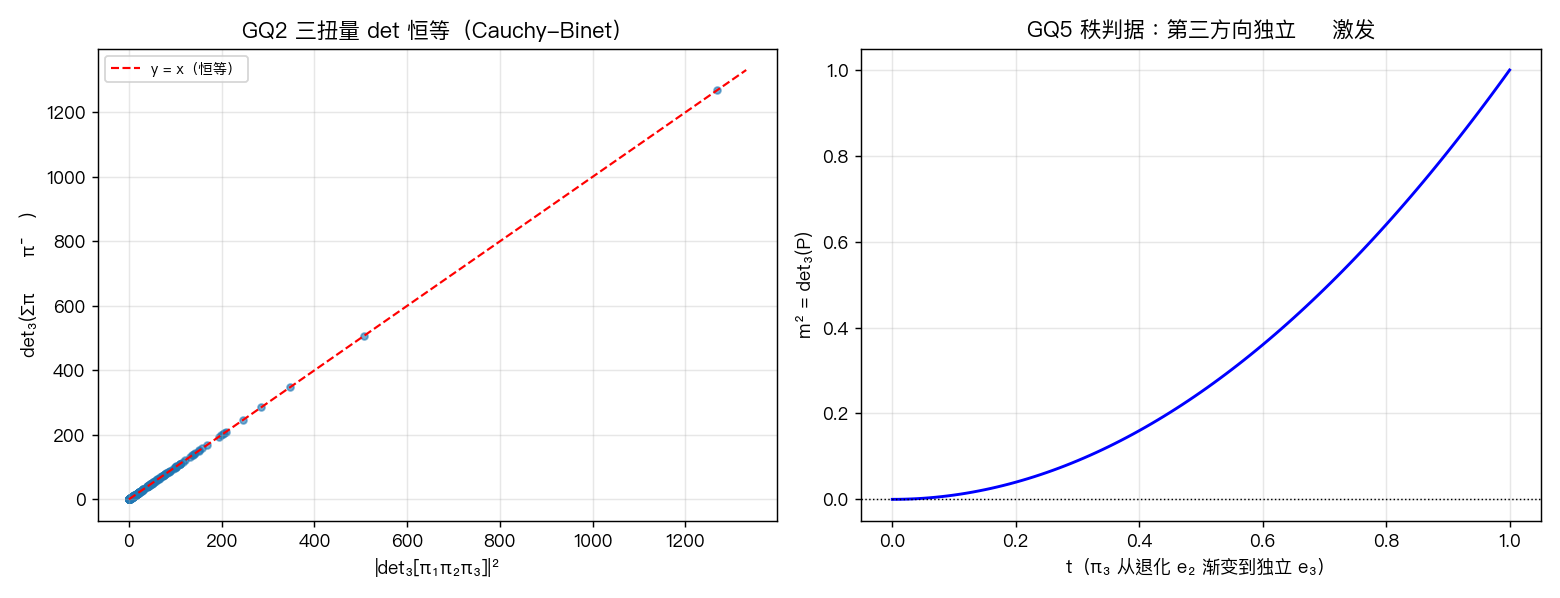
\includegraphics[width=0.9\columnwidth]{figures/fig_triple_rank.png}
\caption{左：$\det_3(P)$ 对 $|\det_3[\pi_1\pi_2\pi_3]|^2$（200 随机样本，
精确恒等）。右：秩扫描——第三方向从退化（$e_2$）渐变到独立（$e_3$），
$m^2$ 从零上升：激发 = 独立第三方向。}
\label{fig:triple}
\end{figure}

\section{信息 = 辛体积：传输、因果、等效速度}
\label{sec:info}

信息被几何地重新定义：\emph{信息 = 辛关联体积} $\det(AA^\dagger)$
（而非密度矩阵熵）。于是：

\paragraph{传输（GQC1）。} 流动的传播算符 $U$ 是酉的（$UU^\dagger=1$），
\begin{equation}
\det\big((UA)(UA)^\dagger\big) = \det(AA^\dagger),
\end{equation}
传输公式 $(UA)(UA)^\dagger = U(AA^\dagger)U^\dagger$。且每个子体积逐项
守恒：$|\det(U A_S)|^2 = |\det A_S|^2$（数值精确）。流动的幺正性 =
辛结构守恒：信息随流传播不衰减。

\paragraph{因果（GQC2）。} 流动是格点局域的：最近邻跳跃矩阵（带宽 1）
$t$ 步后带宽 $\le t$，传播核在格点光锥外为零。因果性从格点局域性涌现
——不可通信定理的几何版，无需额外公设。

\paragraph{等效速度（GQC3）。} 非均匀流动中等效速度 $=1+v_{\rm flow}$：
超光速\emph{等效}运动是几何（坐标拖曳）效应——Alcubierre/Painlev\'e--
Gullstrand 结构——而信号从不超越局部光速。光锥被流动倾斜
（图~\ref{fig:cone}）。

\begin{figure}[htbp]
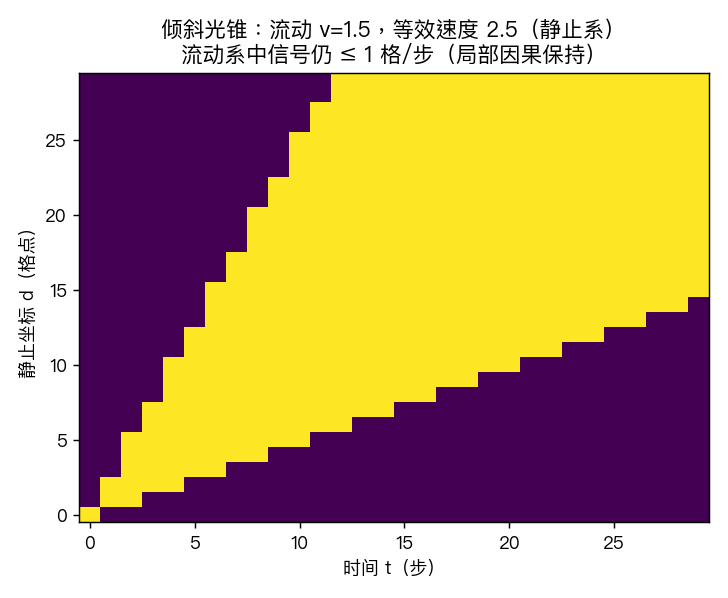
\includegraphics[width=0.9\columnwidth]{figures/fig_tilted_lightcone.png}
\caption{倾斜光锥：流动 $v=1.5$ 时静止系因果区斜率 $1+v$（等效速度
$>1$），而流动系中信号每步 $\le 1$。}
\label{fig:cone}
\end{figure}

\section{四力 = 流动动量的莱布尼茨分解}
\label{sec:forces}

由 $p=m(C-v)$，变化率按莱布尼茨法则分解为四通道（GQF）：
\begin{equation}
\frac{d}{dt}\big[m(C-v)\big]
= \dot m\,C + m\dot C - \dot m\,v - m\dot v ,
\label{eq:fourforces}
\end{equation}
对应电场力（$\dot m C$：质量流 $\times$ 光速方向）、核力（$m\dot C$：
质量 $\times$ 光速流——矢量光速方向变化）、磁场力（$\dot m v$：质量流
$\times$ 速度）与万有引力/惯性力（$m\dot v$：质量 $\times$ 加速度）。
力不是独立实体：它们是流动动量分解的四通道。电荷在同样语言中是空间
位移流的散度：正 = 源（发散右手螺旋），负 = 汇（汇聚右手螺旋）——
图~\ref{fig:charge}。

\begin{figure}[htbp]
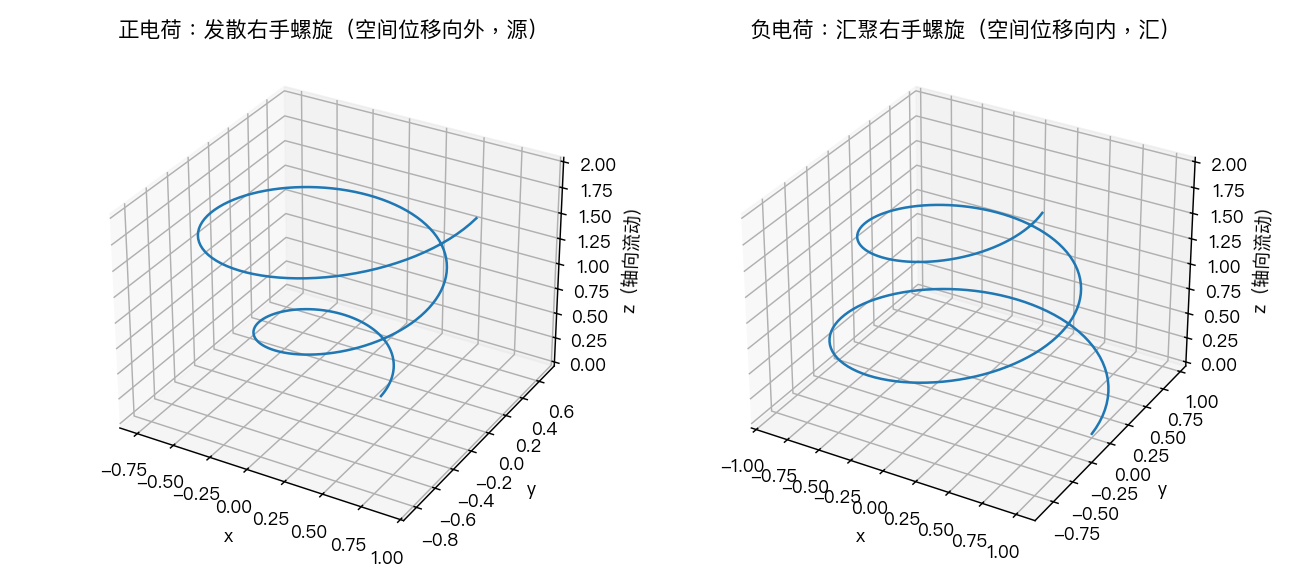
\includegraphics[width=0.9\columnwidth]{figures/fig_charge_helix.png}
\caption{电荷 = 条数流：正电荷 = 发散右手螺旋（源）；负电荷 = 汇聚右手
螺旋（汇）。两者同为右手螺旋；散度区分正负。}
\label{fig:charge}
\end{figure}

\section{光子 = 激发电子螺旋}
\label{sec:photon}

光子是质量与电荷消失的电子激发态：它是电子实体遗留的螺旋结构。
粒子性来自遗留的电子结构；波动性来自空间本身的波动（波动方程的形式化
留作开放）。

两种模型（图~\ref{fig:photon}）：
\begin{itemize}
\item \textbf{模型 A}：一个激发电子做圆柱螺旋运动；直线部分速度为光速。
这是单扭量——秩 1，$\det=0$，无质量（TW1）。
\item \textbf{模型 B}：两个激发电子绕同一轴线对称旋转，沿旋转平面垂直
方向以光速直线运动。环向动量抵消（$p_y+(-p_y)=0$，GQP2），净动量纯
轴向，$E^2=|p|^2$（无质量）：两模型共享同一光锥。
\end{itemize}
光子静止\emph{在}空间中，\emph{随}流动运动（$v=C$：$p=m(C-v)=0$ 且
$m=0$，GQP3）——与流动公设一致。

\begin{figure}[htbp]
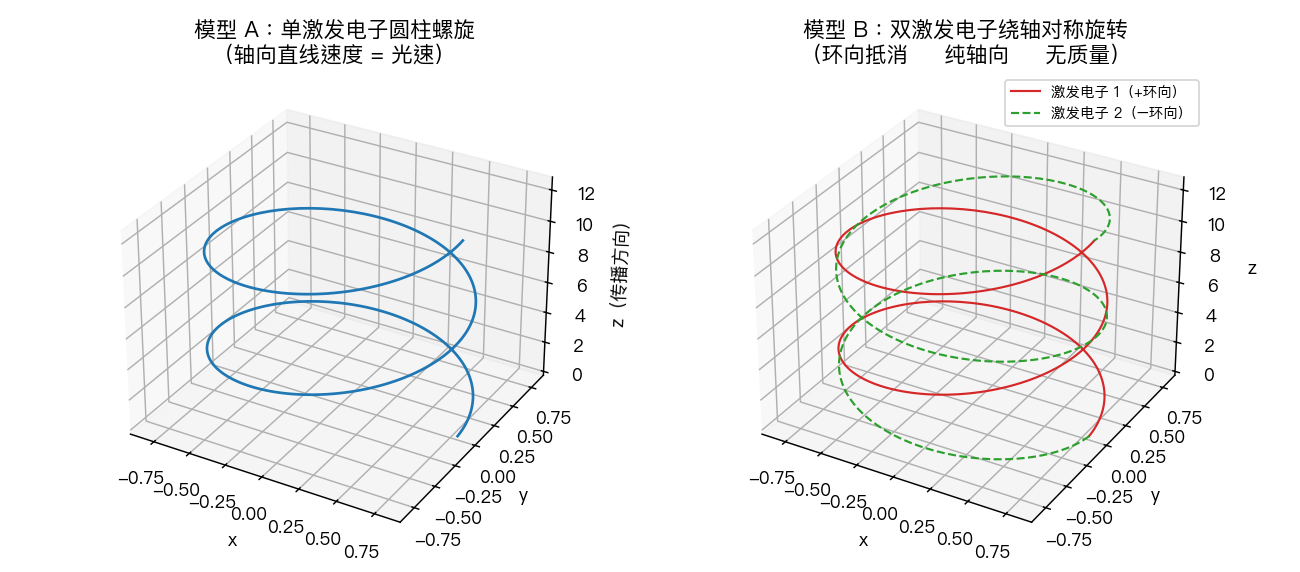
\includegraphics[width=0.9\columnwidth]{figures/fig_photon_models.png}
\caption{光子模型。左：模型 A，单激发电子螺旋（轴向速度 $=c$）。右：
模型 B，双螺旋对称——环向抵消，净动量纯轴向。}
\label{fig:photon}
\end{figure}

\section{量子关系从螺旋几何涌现}
\label{sec:quantum}

\paragraph{能量 = 旋转（GQR）。} 普朗克常数 $h$ = 每圈角动量；约化
普朗克常数 $\hbar=h/2\pi$ = 每弧度角动量。频率 = 每秒圈数（可数的
条数）。于是
\begin{equation}
E = \hbar\omega = \frac{h}{2\pi}\,2\pi f = h\,f =
\underbrace{h}_{\text{每圈角动量}}
\times
\underbrace{f}_{\text{每秒圈数}},
\end{equation}
普朗克-爱因斯坦关系 = 螺旋的旋转能量（图~\ref{fig:turns}）。

\begin{figure}[htbp]
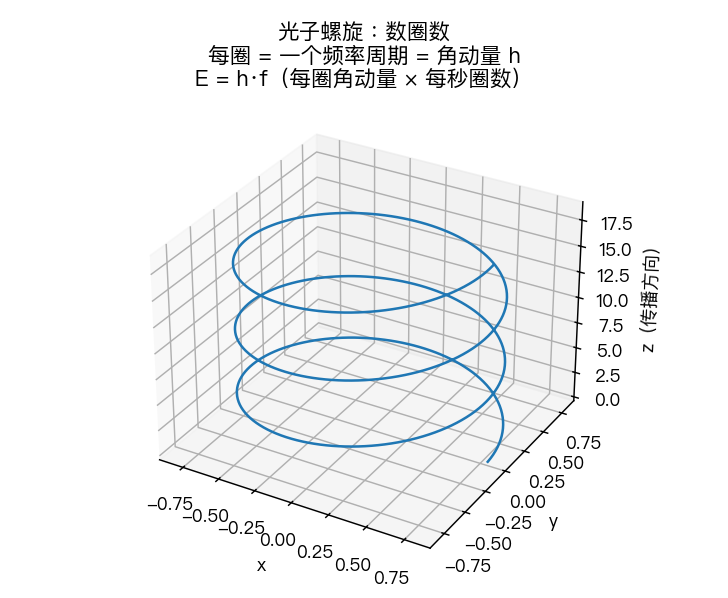
\includegraphics[width=0.9\columnwidth]{figures/fig_photon_turns.png}
\caption{数条数：光子螺旋的每圈 = 一个频率周期 = 角动量 $h$；
$E=h\cdot f$ = 每圈角动量 $\times$ 每秒圈数。}
\label{fig:turns}
\end{figure}

\paragraph{圆周 = 波长（GQR4-6）。} $h$ 与 $\hbar$ 之间的 $2\pi$ 因子
正是螺旋截面的圆周。在几何选择 $r=\lambda/2\pi$（约化波长 = 螺旋半径）
下推导链闭合：
\begin{align}
2\pi r &= \lambda && \text{（一圈 = 一个波长），}\\
\hbar &= r\,p && \text{（角动量 = 半径 $\times$ 动量），}\\
p &= \frac{h}{\lambda} && \text{（德布罗意关系涌现），}\\
E &= pc = hf && \text{（普朗克-爱因斯坦涌现），}
\end{align}
以物理常数代入机器精度验证（表~\ref{tab:circ}）。

\begin{table}[htbp]
\caption{圆周 = 波长：以物理常数闭合推导链（$\lambda=500$\,nm）。}
\label{tab:circ}
\begin{ruledtabular}
\begin{tabular}{lcc}
量 & 数值 & 检验 \\
\hline
$r=\lambda/2\pi$ & $79.58$\,nm & 约化波长 \\
圆周 $2\pi r$ & $500.0$\,nm & $=\lambda$（一圈 = 一个波长） \\
$p=h/\lambda$ & $1.3252\times10^{-27}$\,kg\,m\,s$^{-1}$ & 德布罗意 \\
$\hbar=r\,p$ & $1.0546\times10^{-34}$\,J\,s & 实测 $1.05457\times10^{-34}$；相对误差 $6\times10^{-10}$ \\
$E=pc$ & $3.313\times10^{-19}$\,J & $=hf$ 精确一致 \\
\end{tabular}
\end{ruledtabular}
\end{table}

\section{胶球、夸克与同一个"3"}
\label{sec:glueball}

胶球质量规则读作条数计数：$m=\sqrt{N}\,M_0$，$N=3$ 个锚定方向
（$\sigma_1\sigma_2\sigma_3$）；格点 $N$ 序列 $\{3,6,7\}$（道
$0^{++},2^{++},0^{-+}$）以 $\sqrt{3},\sqrt{6},\sqrt{7}$ 倍 $M_0$ 落入
格点区间。色数 = 同一个"3"：色 $=3$ = 三个空间方向（结构对应：
为什么 3 色）；8 胶子 $= 2^3 = \dim C\ell(6)$（TW5）。空间的"3"、
色的"3"与胶球锚定的"3"是同一结构。

诚实边界：夸克质量谱（$2.2$\,MeV $\to$ $173$\,GeV）无条数规律——
夸克质量是 QCD 自由参数；色条数只给结构不给数值。

\section{数值验证}
\label{sec:validation}

以上全部恒等经数值验证（N1--N29，机器精度）：Cauchy--Binet 链
（$\le 5.9\times10^{-12}$）、酉传输（公式误差 $0$，子体积逐项守恒
$\le 5.9\times10^{-12}$）、光锥带宽（违规 $0$）、四力分解（误差 $0$）、
光子模型（环向抵消 $0$）、量子匹配（$E=\hbar\omega$ 相对误差 $0$；
$\hbar=rp$ 相对误差 $6\times10^{-10}$；$E=pc$ 对 $E=hf$ 误差 $0$）、
"3"链条（正交单位方向 $\det_3=1$，$m=\sqrt3\,M_0$）。

\section{诚实评估}
\label{sec:honest}

以下是被声称的，以及未被声称的。

\paragraph{已声称。} (i) 从单一原初实体（流动空间）出发的一条自洽链
覆盖质量、信息、因果、等效速度、力、光子与量子关系；(ii) 推导
\emph{链已闭合}：在几何选择 $r=\lambda/2\pi$ 下，德布罗意与
普朗克-爱因斯坦关系是螺旋几何加经典恒等的推论；(iii) 全部陈述在
Lean 4 中零 \texttt{sorry} 形式化，数值机器精度验证。

\paragraph{未声称。} (i) 几何选择 $r=\lambda/2\pi$ 的第一性推导（其来源
未知）；(ii) 剩余常数的数值推导：$G$ 与 $e$ 是\emph{结构性存在}——
$G$ = 雨速公式 $v(r)=\sqrt{2GM/r}$ 中的流动梯度常数（视界处 $v=c$，
精确），$e$ = 条数流率量子，精细结构常数
$\alpha=e^2/(4\pi\varepsilon_0\hbar c)=1/137.036$ 是 $e$、$\hbar$、$c$
的几何比（验证到 $6\times10^{-10}$）——但它们的数值仍依赖 $M_0$
标定与实测 $\alpha$；(iii) 标准框架之外的任何新的可证伪预言（格点
$N$ 序列是后验拟合）；(iv) 光子波动性的连续波动方程、电荷散度形式
仍是形式化骨架。

\section{结论}
\label{sec:conclusion}

流动空间框架以一条精确恒等链统一了物理长期分开的概念：质量（辛体积）、
信息（还是辛体积）、因果（格点局域性）、力（流动动量的莱布尼茨通道）、
光子（激发电子螺旋）与量子关系（螺旋的旋转；圆周 = 波长）。链已闭合；
链首的几何选择是开放问题。基座能否存活是实验的问题；框架现在已足够
精确到可以被证伪。

\end{document}
